\section{SplatAnything}
\label{sec:method}

\subsection{Formulation}

Given $N$ input images
$\mathcal{I}=\{I_i\}_{i=1}^{N}$,
together with optional camera intrinsics
$\mathcal{K}=\{K_i\}_{i=1}^{N}$
and extrinsics
$\mathcal{T}=\{(R_i,t_i)\}_{i=1}^{N}$,
our goal is to predict a 3D Gaussian scene representation
\begin{equation}
    \mathcal{G}
    =
    \left\{
        \left(\mu_j,\alpha_j,\Sigma_j,\mathrm{sh}_j\right)
    \right\}_{j=1}^{M},
\end{equation}
where $\mu_j$, $\alpha_j$, $\Sigma_j$, and $\mathrm{sh}_j$
denotethe Gaussian center, opacity, covariance, and SH coefficients.


\subsection{Preliminaries}

\paragraph{Gaussian spacing.}
For per-pixel Gaussian prediction, each valid image pixel defines a
Gaussian center at its back-projected 3D point. We refer to the spatial
spacing between Gaussian centers induced by neighboring image pixels as
\emph{Gaussian spacing}. This quantity is particularly relevant to
Gaussian-scale prediction, since adequate surface coverage requires the
Gaussian scale to be commensurate with the local Gaussian spacing.

For the $i$-th view, let $D_i(\mathbf{u})$ denote the depth at pixel
$\mathbf{u}=(u,v)$, and let $(f_{x,i},f_{y,i})$ and
$(c_{x,i},c_{y,i})$ denote the focal lengths and principal point in
pixels. Under the pinhole camera model, the back-projected point $\mathbf{P}_i^{c}(\mathbf{u})$ in the
local camera frame is
\begin{equation}
    \mathbf{P}_i^{c}(\mathbf{u})
    =
    D_i(\mathbf{u})
    \begin{bmatrix}
        (u-c_{x,i})/f_{x,i} \\
        (v-c_{y,i})/f_{y,i} \\
        1
    \end{bmatrix}.
    \label{eq:back_projection}
\end{equation}

Consider two horizontally adjacent pixels $\mathbf{u}$ and
$\mathbf{u}+\mathbf{e}_x$. Under a locally constant-depth approximation,
$D_i(\mathbf{u}+\mathbf{e}_x)\approx D_i(\mathbf{u})$, their horizontal
Gaussian spacing is
\begin{equation}
    d_{x,i}(\mathbf{u})
    =
    \left\|
        \mathbf{P}_i^{c}(\mathbf{u}+\mathbf{e}_x)
        -
        \mathbf{P}_i^{c}(\mathbf{u})
    \right\|_2
    \approx
    \frac{D_i(\mathbf{u})}{f_{x,i}}.
    \label{eq:horizontal_gaussian_spacing}
\end{equation}
Similarly, the vertical spacing is
$d_{y,i}(\mathbf{u})\approx D_i(\mathbf{u})/f_{y,i}$.
We summarize the two directions using their geometric mean,
\begin{equation}
    d_i(\mathbf{u})
    =
    \sqrt{
        d_{x,i}(\mathbf{u})d_{y,i}(\mathbf{u})
    }
    \approx
    \frac{D_i(\mathbf{u})}
    {\sqrt{f_{x,i}f_{y,i}}},
    \label{eq:gaussian_spacing}
\end{equation}
which we use as a first-order scalar characterization of local Gaussian
spacing.


\subsection{Normalization Space for Gaussian Prediction}
\label{sec:gsnorm}

\paragraph{Limitation of radial distance normalization.}

Feed-forward 3DGS methods built on geometry foundation models typically
predict Gaussian attributes in the normalized coordinate space inherited
from their geometry backbones. These models commonly normalize a reconstructed scene using the mean radial distance of 3D points to the reference-camera origin, which we
refer to as \emph{Radial Distance Normalization (RDNorm)}.
Let $\mathbf{P}_i(\mathbf{u})$ denote the reconstructed 3D point at
pixel $\mathbf{u}$ in view $i$, expressed in the reference-camera
coordinate system before scene-level normalization, and let $\Omega_i$
denote the set of valid pixels in view $i$.
The normalization factor $s_r$ under RDNorm is computed as
\begin{equation}
    s_r
    =
    \frac{1}{N_p}
    \sum_{i=1}^{N}
    \sum_{\mathbf{u}\in\Omega_i}
    \left\|
        \mathbf{P}_i(\mathbf{u})
    \right\|_2,
    \qquad
    N_p
    =
    \sum_{i=1}^{N}|\Omega_i|.
    \label{eq:radial_distance}
\end{equation}

\begin{figure}[t]
    \centering
    \includegraphics[width=\textwidth]{figures/method/pipeline_2.jpg}
    \vspace{-0.2in}
    \caption{
        \textbf{Architecture of SplatAnything.}
        Given $N$ input images and optional camera parameters,
        a frozen geometry foundation model first estimates multi-view
        geometry.
        We convert the geometry from its native radial-distance-normalized
        space to the proposed Gaussian-spacing-normalized space and predict
        per-pixel Gaussian attribute through a Gaussian backbone and a lightweight GShead.
    }
    \label{fig:architecture}
    \vspace{-0.12in}
\end{figure}

The geometry, depth, and camera translations are then rescaled as
\begin{equation}
    \mathbf{P}_i^{r}
    =
    \frac{\mathbf{P}_i}{s_r},
    \qquad
    D_i^{r}
    =
    \frac{D_i}{s_r},
    \qquad
    \mathbf{t}_i^{r}
    =
    \frac{\mathbf{t}_i}{s_r},
    \label{eq:rdnorm}
\end{equation}


From Eq.~\ref{eq:gaussian_spacing}, the Gaussian spacing after RDNorm is
approximately
\begin{equation}
    d_i^{r}(\mathbf{u})
    \approx
    \frac{D_i^{r}(\mathbf{u})}
    {\sqrt{f_{x,i}f_{y,i}}}
    =
    \frac{D_i(\mathbf{u})}
    {\sqrt{f_{x,i}f_{y,i}}\,s_r}.
    \label{eq:rdnorm_spacing}
\end{equation}

RDNorm canonicalizes a scene-level radial statistic of the reconstructed geometry, but does not directly canonicalize a scene-level statistic of Gaussian spacing.

\begin{wrapfigure}[16]{r}{0.42\linewidth}
    \centering
    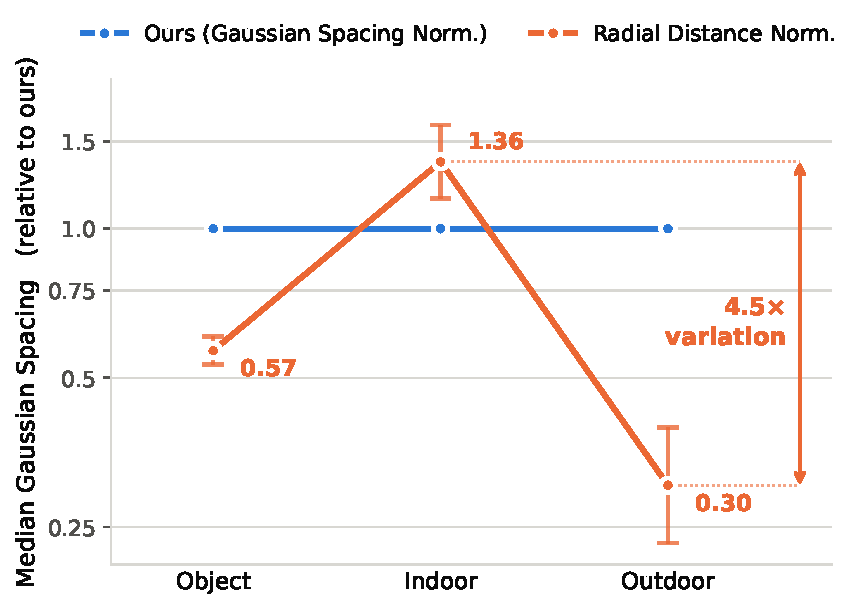
\includegraphics[width=\linewidth]{figures/method/point_spacing.pdf}
    \vspace{-0.25in}
    \caption{
        \textbf{Median Gaussian spacing across scene types.}
        RDNorm leaves up to $4.5\times$ variation in median Gaussian spacing
        across scene categories, whereas GSNorm canonicalizes it by
        construction.
    }
    \vspace{-0.1in}
    \label{fig:point_spacing_comparison}
\end{wrapfigure}

Consequently, the spacing between neighboring Gaussian centers can still
vary substantially across different scene scales and camera
configurations, as shown in
Fig.~\ref{fig:point_spacing_comparison}.
This variation is particularly
important for Gaussian prediction because the Gaussian scale required
for adequate surface coverage should be commensurate with the local
Gaussian spacing. Therefore, similar local observations can correspond
to different Gaussian-scale targets after RDNorm,
introducing ambiguity in scale supervision across scenes. This motivates us to
define the normalization space directly from a representative statistic
of Gaussian spacing.


% \vspace{-0.05in}
\paragraph{Gaussian spacing normalization.}
% \vspace{-0.05in}
We propose \emph{Gaussian Spacing Normalization (GSNorm)}, which
defines the coordinate scale for Gaussian prediction using Gaussian spacing
rather than a global radial statistic.
Because the reconstruction is rescaled by a single scene-level factor,
we use the median characteristic Gaussian spacing as a robust representative
scale.
Specifically, for a generic scene-level scale $s>0$, the characteristic
Gaussian spacing becomes
\begin{equation}
    d_i^{s}(\mathbf{u})
    \approx
    \frac{D_i(\mathbf{u})}
    {\sqrt{f_{x,i}f_{y,i}}\,s}.
\end{equation}
GSNorm chooses $s$ such that the scene-level median Gaussian spacing is
canonicalized:
\begin{equation}
    \operatorname*{median}_{i,\mathbf{u}\in\Omega_i}
    \left(
        d_i^{s}(\mathbf{u})
    \right)
    \approx
    \operatorname*{median}_{i,\mathbf{u}\in\Omega_i}
    \left(
        \frac{D_i(\mathbf{u})}
        {\sqrt{f_{x,i}f_{y,i}}\,s}
    \right)
    =
    1.
    \label{eq:gsnorm_objective}
\end{equation}

Since the median is equivariant to positive scaling,
Eq.~\ref{eq:gsnorm_objective} directly yields the normalization factor $s_g$:
\begin{equation}
    s_g
    =
    \operatorname*{median}_{i,\mathbf{u}\in\Omega_i}
    \left(
        \frac{D_i(\mathbf{u})}
        {\sqrt{f_{x,i}f_{y,i}}}
    \right).
    \label{eq:gs_scale}
\end{equation}

Using $s_g$, we rescale the geometry, depth, and camera translations as
\begin{equation}
    \mathbf{P}_i^{g}
    =
    \frac{\mathbf{P}_i}{s_g},
    \qquad
    D_i^{g}
    =
    \frac{D_i}{s_g},
    \qquad
    \mathbf{t}_i^{g}
    =
    \frac{\mathbf{t}_i}{s_g}.
    \label{eq:gsnorm}
\end{equation}

GSNorm canonicalizes the scene-level median Gaussian spacing while preserving
the relative variation of local Gaussian spacing.
This aligns the representative Gaussian spacing scale across scenes and camera
configurations without suppressing meaningful local geometric variation.
Compared with RDNorm, GSNorm therefore provides a more consistent scale
reference for Gaussian prediction that is directly related to Gaussian
surface coverage.
This alleviates ambiguity in Gaussian-scale supervision across different
input settings, facilitating the learning of a feed-forward Gaussian
model with robust cross-scene and cross-view generalization.

% \vspace{-0.1in}
\subsection{SplatAnything Architecture}
\label{sec:architecture}
% \vspace{-0.08in}
The overall architecture is illustrated in
Fig.~\ref{fig:architecture}. More details are provided in the appendix.

% \vspace{-0.1in}

\paragraph{Geometry prediction and rescaling.}

Given $N$ input images and optional camera parameters, we employ the
frozen WorldMirror~2.0~\citep{team2026hy} geometry model to estimate
multi-view depths, intrinsics, and camera poses. The predicted depths
and camera translations are initially represented in the
radial-distance-normalized coordinate space of the geometry model.
We then use GSNorm (Eq.~\ref{eq:gsnorm}) to rescale these
scale-dependent quantities into the proposed Gaussian-spacing-normalized
space, obtaining
$D^{g}=\{D_i^{g}\}_{i=1}^{N}$ and
$T^{g}=\{(R_i,t_i^{g})\}_{i=1}^{N}$.
We unproject the rescaled depth maps using the corresponding camera
parameters to obtain
$\mathbf{P}^{g}=\{\mathbf{P}_i^{g}\}_{i=1}^{N}$,
where each valid per-pixel 3D point serves as the center of a Gaussian
primitive.
% \vspace{-0.1in}

\paragraph{Gaussian attribute prediction.}

We initialize a \emph{Gaussian Backbone} from the geometry backbone
of WorldMirror~2.0 and fine-tune it for Gaussian prediction.
A lightweight \emph{GSHead}, trained from scratch, predicts
per-pixel Gaussian attributes for all input views:
\begin{equation}
    \{\mathcal{G}_i^{g}\}_{i=1}^{N}
    =
    \mathrm{GSHead}
    \left(
        \mathrm{GaussianBackbone}(\mathcal{I}, Optional\mathcal{(K, T)})
    \right).
\end{equation}

For each pixel, the network predicts opacity, rotation, scale,
and spherical-harmonic appearance coefficients.
Together with the corresponding center from $\mathbf{P}^{p}$,
these quantities define the per-pixel Gaussian primitives in the
Gaussian-spacing-normalized coordinate space.


% \paragraph{Gaussian Merging.}

% Following AnySplat~\citep{jiang2025anysplat}, we predict a per-pixel
% weight map
% $w^{p}=\{w_i^{p}\}_{i=1}^{N}$
% and merge redundant per-view Gaussians within local voxels.
% This produces the final unified 3D Gaussian scene representation
% $\mathcal{G}$.

% \vspace{-0.1in}


\subsection{Training SplatAnything}
\label{sec:training}
The training datasets and view-sampling strategies are detailed in the
appendix.

Given a rendered target-view image $\hat{I}_t$ and its ground-truth
image $I_t$, we supervise the model using a pixel-wise MSE loss and an
LPIPS perceptual loss:
\begin{equation}
    \mathcal{L}_{\mathrm{MSE}}
    =
    \frac{1}{3HW}
    \left\|
        \hat{I}_t-I_t
    \right\|_2^2,
    \qquad
    \mathcal{L}_{\mathrm{LPIPS}}
    =
    \operatorname{LPIPS}
    \left(
        \hat{I}_t,I_t
    \right).
\end{equation}

The overall objective is
\begin{equation}
    \mathcal{L}
    =
    \lambda_{\mathrm{MSE}}
    \mathcal{L}_{\mathrm{MSE}}
    +
    \lambda_{\mathrm{LPIPS}}
    \mathcal{L}_{\mathrm{LPIPS}},
\end{equation}
where
$\lambda_{\mathrm{MSE}}=\lambda_{\mathrm{LPIPS}}=1$
in our implementation.

SplatAnything is trained for 20,000 iterations on 64 NVIDIA H20 GPUs,
using 4 to 32 input views and dynamically varying the input resolution
from 504 to 1024. We use a 500-step warm-up and learning rates of
$5\times10^{-6}/2\times10^{-5}$ for the
Gaussian Backbone and GSHead.